\part{Projekt Management}

\section{Management von Softwareprojekten}

\paragraph{Eine Organisation} kann definiert werden über ihre Struktur, ihre Funktion oder die Institution, welche sie darstellt.

\paragraph{Das Management} übernimmt Leitungsaufgaben in Projekten und Unternehmen. Es handelt sich um eine Gruppe von Personen welche sich mit typischen Aufgaben wie Planung, Delegation, Organisation sowie Führung und Erfolgskontrolle. 

\paragraph{Ein Artefakt} ist ein primäres oder sekundäres Arbeitsergebnis, welches durch Projektaktivitäten erstellt wird. Beispiele: Pflichtenheft, Architekturentwurf, Testfallbeschreibung. 

\paragraph{Ein Projekt} ist komplex, neuartig, zeitlich befristet und weist begrenzte Ressourcen / Budget, Teamarbeit und messbare Ziele und Ergebnisse auf. Projektbeispiele sind ein neu entwickeltes, lauffähiges Softwaresystem, Teilergebnisse für die Entwicklung von Software, die Migration einer Software auf eine andere 
Hardwareplattform. 
Keine Projekte sind Routinetätigkeiten, Vorhaben des "daily business" wie beispielsweise Archivverwaltung und Kantinenbewirtschaftung. 
Ein Grenzbereich könnte die Pflege der Datenverarbeitung darstellen. 

Softwareentwicklungsprojekte unterscheiden sich nicht grundlegend zu anderen Entwicklungsprojekten wie Elektrotechnische Erzeugnisse, Maschinen und Bauwerke. Es gibt jedoch einige signifikante Unterschiede durch die \emph{Immaterialität} (Abstraktes Artefakt, bei SW nur Entwicklungsprozesse und 
Inbetriebnahme und keinen wirklichen Produktions- bzw. Fertigungsprozess). Die Folge davon ist, dass Fehler bei materiellen Produkten in der Regel noch während Planung oder Durchführung der Fertigung erkannt werden. 

\paragraph{Projektstatistiken}
Gemäss der CHAOS 2004 Umfrage kam es 2005 zu 15.52\% und 2007 zu 11.54\% Projektabbrüchen. Die Statistiken zeigen einen Trend, sollten jedoch nicht absolut verglichen werden. Gemäss der Standish Group sind die Zahlen nicht glaubhaft (``Nur weil jemand eine Frage stellt, bedeutet das nicht, dass wir antworten. Tatsächlich antworten wir eher nicht'')


\paragraph{Gescheiterte Software Projekte}
Der Ariane 5 Fehlstart.
Am 4. Juni 1996 startete die Ariane 5 Rakete zu ihrem Erstflug. Nach genau 36,7 Sekunden sprengte sich die Rakete selbst inklusive vier Satelliten. Kosten: 500 Mio Dollar. Ursache: 64Bit zu 16Bit-Wandlung.

\subsection{Ziele des Managements}
Die Ziele des Software Engineering sind ein Produkt kostengünstig, termingerecht und in angemessener Qualität anzuliefern. Teilziele sind die Beherrschung von Zeit und Kosten. Kann ein unterschiedlicher Fokus gelegt werden: kostenfixiert, terminfixiert, leistungsfixiert, mit dem Ziel der Erreichung von Qualitätszielen, der Sicherung von Investitionen oder der Einhaltung von Rahmenbedingungen. Folgender Zusammenhang gilt zwischen den Fehlerkosten von Softwareprojekten:
\begin{figure}[hb]
    \centering
    % \adjustbox{width=10cm}{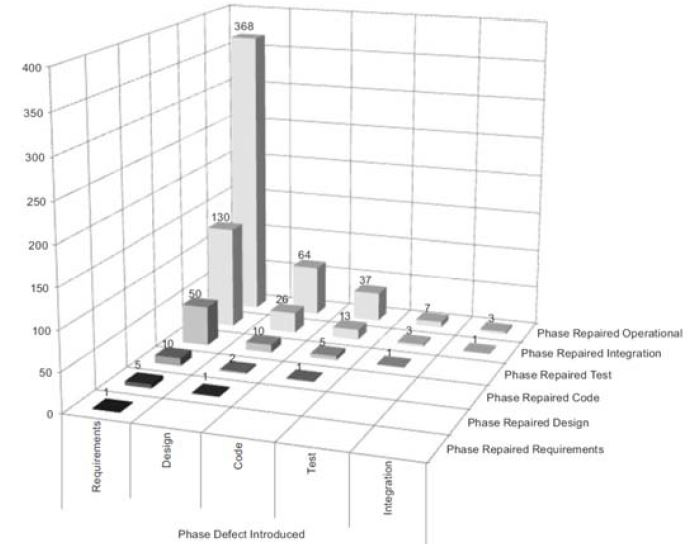
\includegraphics{Figures/bugfixingcost}}
\caption[]{Relative Bugfixing Kosten}
\end{figure}

\paragraph{Faktoren für erfolgreiche Projekte sind}
\begin{itemize}
    \item Angestellte: Hohe Motivation der Mitarbeiter / Erfahrene  Projektmanager und Entwickler 
    \item Kundenorientierung 
    \item Management: Klare Projektziele / Realistische Projektpläne / Klare Verantwortungsstrukturen / Offene Kommunikationskultur 
    \item Prozessorientierung 
    \item Dokumentation und Artefakte 
    \item Modularisierung und Wiederverwendung
\end{itemize}


\section{Produkt-, Projekt- und Softwarelebenszyklus}
Der Softwarelebenszyklus ist als Spezialisierung des Produktlebenszyklus anzusehen.
\begin{figure}[ht]
    \centering
    % \adjustbox{width=11cm}{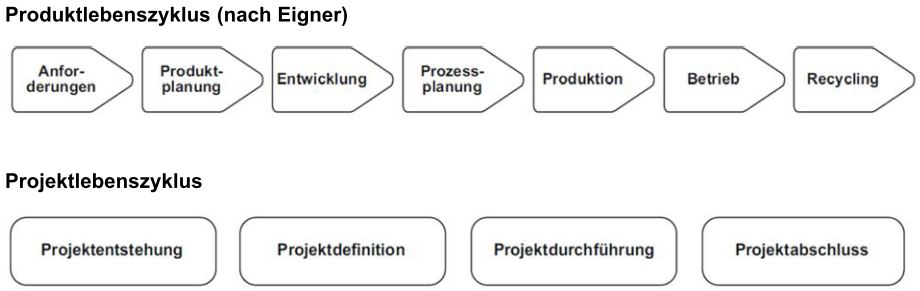
\includegraphics{Figures/lebenszyklus}}
    \caption[]{Produkt- \& Projektlebenszyklus}
\end{figure}


\subsection{Softwarelebenszyklus}
\begin{itemize}
    \item Analyse: Anforderungsfestlegung
    \item Design: Grob- \& Feinentwurf (Architektur, Programmstruktur)
    \item Implementierung
    \item Test und Integration
    \item Betrieb \& Wartung: Erprobung und Inbetriebnahme sowie Wartung und Weiterentwicklung
    \item Ausserbetriebnahme
\end{itemize}
Der Softwarelebenszyklus muss nicht sequentiell ablaufen. Zudem kann der Prozess iterativ mehrmals durchlaufen werden. 

\subsection{Phasen im Projektlebenszyklus}
\begin{itemize}
    \item Projektentstehung
    \begin{enumerate}
        \item Projektidee entwickeln: Ziele, Bedarf, Chancen festlegen \& ggf. Projektvorstudie durchführen \(\rightarrow\) \textbf{M1: Projektskizze}
        \item Aufwand schätzen sowie Anforderungen und Ziele grob festlegen: Anforderungen notieren, grober Plan definieren, Schätzung durchführen und in einem Business Case zusammenfassen \(\rightarrow\) \textbf{M2: Projektauftrag}
        \item Angebots- und Vertragswesen: Lastenheft und Angebot festlegen und Gegenpartei übergeben \(\rightarrow\) \textbf{M3: Vertrag / Projektvereinbarung}
    \end{enumerate}
    \item Projektdefinition
    \begin{enumerate}
        \item Projekt strukturieren und Projektteam organisieren
        \item Definition eines Projektmanagementverfahrens und Erstellen eines Projekthandbuchs
        \item Definition eines QS-Verfahrens und Erstellen eines QS-Handbuch
        \item Aufbau einer Projektinfrastruktur
        \item Projekt planen bzw. Erstellen eines Projektplan
    \end{enumerate}
    \item Projektdurchführung:
    Durchführung eines iterativen Entwicklungsprozess gemäss den Phasen des V-Modells. Der Input entspricht dem Pflichtenheft und die Lieferung dem Output. Zeitgleich werden die iterativen Phasen von Planung (Soll-Vorhaben) \(\rightarrow\) Kontrolle  (Messung von Kennzahlen und Soll- / Ist-Vergleich) \(\rightarrow\) Steuerung (Steuerungsmasssnahmen hinsichtlich QS oder Projektmanagement) \(\rightarrow\) Anpassung des Vorhabens durchlaufen.
    \begin{itemize}
        \item Erfassung und Verfeinerung der Anforderungen
        \item Systementwurf
        \item Implementierung, Verifikation und Test
        \item Test und Integration
        \item Erprobung und Übergabe
    \end{itemize}
    \item Projektabschluss
    \begin{enumerate}
        \item Ergebnisse der Entwicklung: Code, Systemarchitektur, Tests, Dokumentation, System
        \item Lieferung abnehmen und System in Betrieb setzen (inkl. Freigaben)
        \item Projekt abschliessen beinhaltet die Sicherung der gemachten Erfahrungen, die Auflösung des Projektteams und die Projektabrechnung \(\rightarrow\) Projektabschlussbericht
    \end{enumerate}
\end{itemize}
Mx: stehen für die erreichten Meilensteine innerhalb einer Phase

% 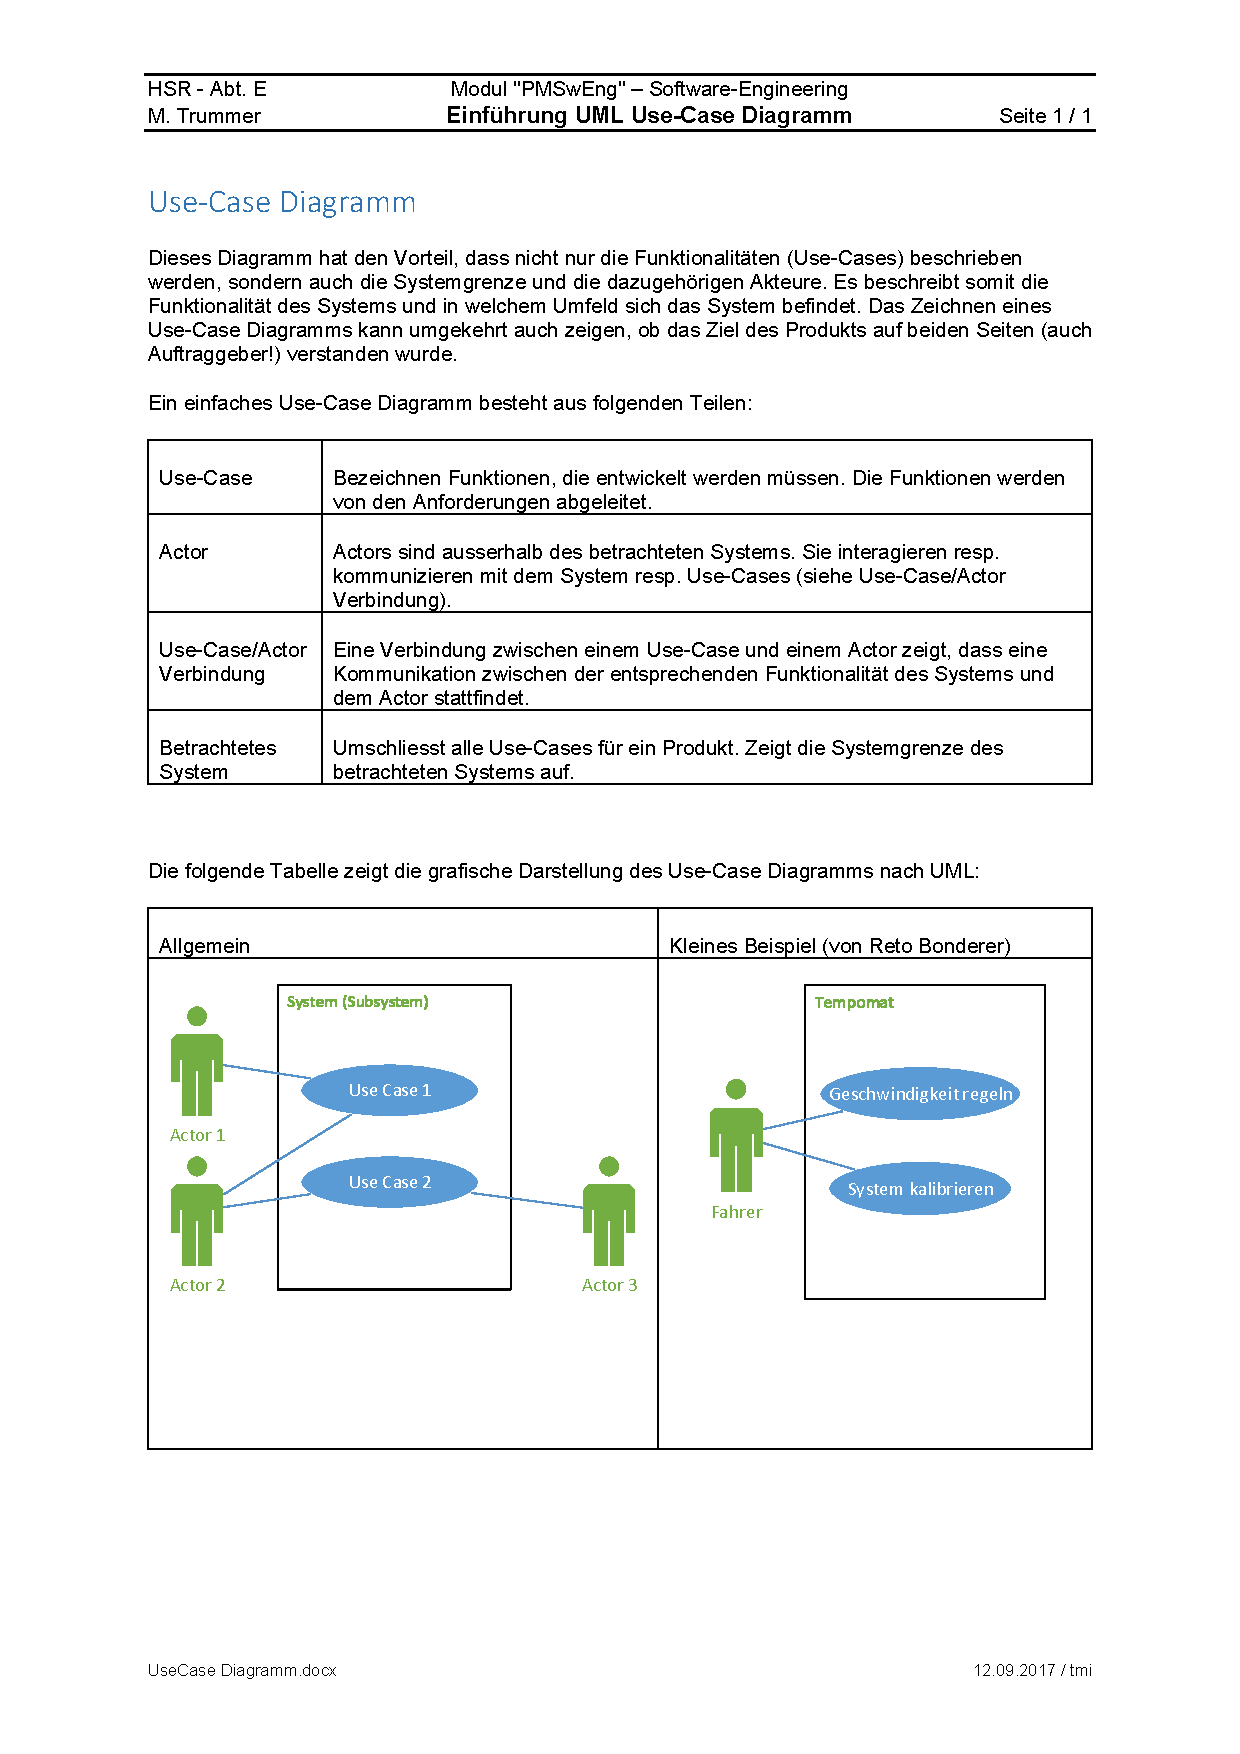
\includepdf[pages=-]{./Uebungen/UseCaseDiagramm.pdf}
